\documentclass[11pt,a4paper]{report}
\usepackage[textwidth=37em,vmargin=30mm]{geometry}
\usepackage{calc,xunicode,amsmath,amssymb,paralist,enumitem,tabu,booktabs,datetime2,xeCJK,xeCJKfntef,listings}
\usepackage{tocloft,fancyhdr,tcolorbox,xcolor,graphicx,eso-pic,xltxtra,xelatexemoji}

\newcommand{\envyear}[0]{2025}
\newcommand{\envdatestr}[0]{2025-10-27}
\newcommand{\envfinaldir}[0]{webdb/2025/20251027/final}

\usepackage[hidelinks]{hyperref}
\hypersetup{
    colorlinks=false,
    pdfpagemode=FullScreen,
    pdftitle={Web Digest - \envdatestr}
}

\setlength{\cftbeforechapskip}{10pt}
\renewcommand{\cftchapfont}{\rmfamily\bfseries\large\raggedright}
\setlength{\cftbeforesecskip}{2pt}
\renewcommand{\cftsecfont}{\sffamily\small\raggedright}

\setdefaultleftmargin{2em}{2em}{1em}{1em}{1em}{1em}

\usepackage{xeCJK,xeCJKfntef}
\xeCJKsetup{PunctStyle=plain,RubberPunctSkip=false,CJKglue=\strut\hskip 0pt plus 0.1em minus 0.05em,CJKecglue=\strut\hskip 0.22em plus 0.2em}
\XeTeXlinebreaklocale "zh"
\XeTeXlinebreakskip = 0pt


\setmainfont{Brygada 1918}
\setromanfont{Brygada 1918}
\setsansfont{IBM Plex Sans}
\setmonofont{JetBrains Mono NL}
\setCJKmainfont{Noto Serif CJK SC}
\setCJKromanfont{Noto Serif CJK SC}
\setCJKsansfont{Noto Sans CJK SC}
\setCJKmonofont{Noto Sans CJK SC}

\setlength{\parindent}{0pt}
\setlength{\parskip}{8pt}
\linespread{1.15}

\lstset{
	basicstyle=\ttfamily\footnotesize,
	numbersep=5pt,
	backgroundcolor=\color{black!5},
	showspaces=false,
	showstringspaces=false,
	showtabs=false,
	tabsize=2,
	captionpos=b,
	breaklines=true,
	breakatwhitespace=true,
	breakautoindent=true,
	linewidth=\textwidth
}






\newcommand{\coverpic}[2]{
    % argv: itemurl, authorname
    Cover photo by #2~~(\href{#1}{#1})
}
\newcommand{\makeheader}[0]{
    \begin{titlepage}
        % \newgeometry{hmargin=15mm,tmargin=21mm,bmargin=12mm}
        \begin{center}
            
            \rmfamily\scshape
            \fontspec{BaskervilleF}
            \fontspec{Old Standard}
            \fontsize{59pt}{70pt}\selectfont
            WEB\hfill DIGEST
            
            \vfill
            % \vskip 30pt
            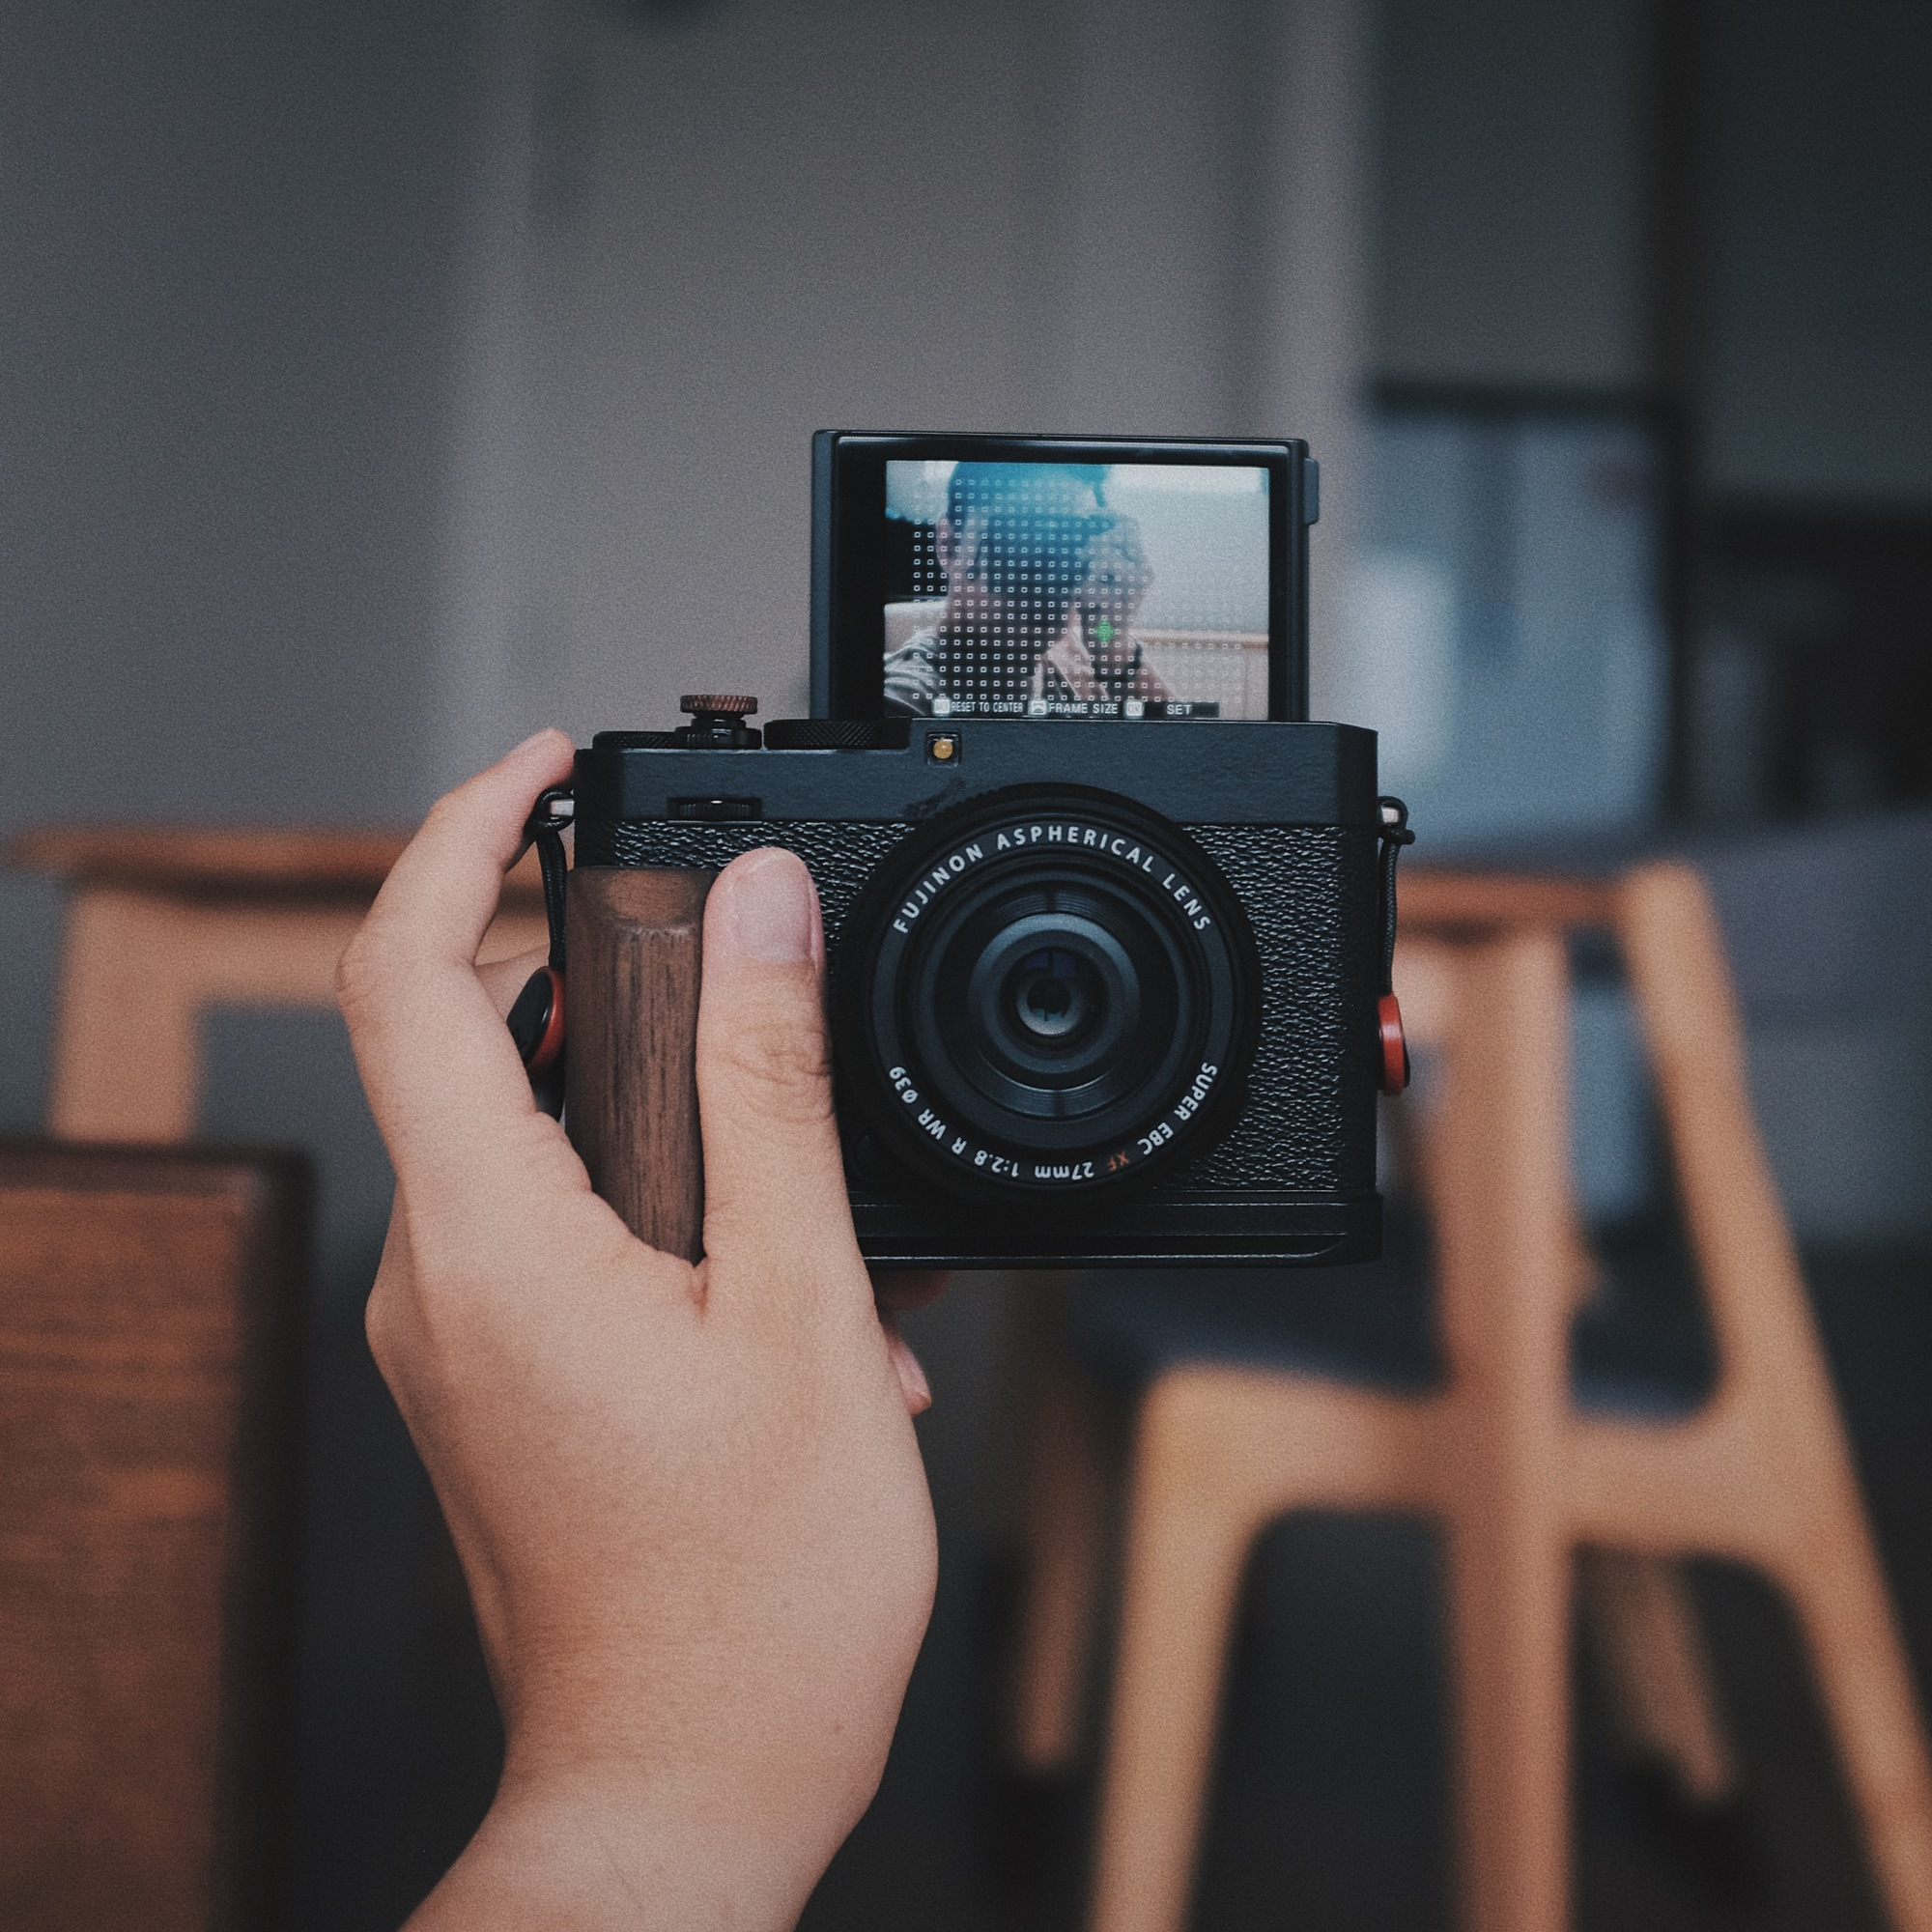
\includegraphics[width=\linewidth]{\envfinaldir/coverpic-prod.jpg}\par
            % \vskip 30pt
            \vfill

            \normalsize\rmfamily\scshape
            \copyright{} The Web Digest Project \hfill\large \envdatestr
        \end{center}
    \end{titlepage}
    % \restoregeometry
}
\newcommand{\simplehref}[1]{%
    \textcolor{blue!80!green}{\href{#1}{#1}}%
}
\renewcommand{\contentsname}{\center\Huge\sffamily\bfseries Contents\par\vskip 20pt}
\newcounter{ipartcounter}
\setcounter{ipartcounter}{0}
\newcommand{\ipart}[1]{
    % \vskip 20pt
    \clearpage
    \stepcounter{ipartcounter}
    \phantomsection
    \addcontentsline{toc}{chapter}{#1}
    % \begin{center}
    %     \Huge
    %     \sffamily\bfseries
    %     #1
    % \end{center}
    % \vskip 20pt plus 7pt
}
\newcounter{ichaptercounter}
\setcounter{ichaptercounter}{0}
\newcommand{\ichapter}[1]{
    % \vskip 20pt
    \clearpage
    \stepcounter{ichaptercounter}
    \phantomsection
    \addcontentsline{toc}{section}{\numberline{\arabic{ichaptercounter}}#1}
    \begin{center}
        \Huge
        \sffamily\bfseries
        #1
    \end{center}
    \vskip 20pt plus 7pt
}
\newcommand{\entrytitlefont}[1]{\subsection*{\raggedright\Large\sffamily\bfseries#1}}
\newcommand{\entryitemGeneric}[2]{
    % argv: title, url
    \parbox{\linewidth}{
        \entrytitlefont{#1}\par\vskip 5pt
        \footnotesize\ttfamily\mdseries
        \simplehref{#2}
    }\vskip 11pt plus 11pt minus 1pt
}
\newcommand{\entryitemGithub}[3]{
    % argv: title, url, desc
    \parbox{\linewidth}{
        \entrytitlefont{#1}\par\vskip 5pt
        \footnotesize\ttfamily\mdseries
        \simplehref{#2}\par\vskip 5pt
        \small\rmfamily\mdseries#3
    }\vskip 11pt plus 11pt minus 1pt
}
\newcommand{\entryitemAp}[3]{
    % argv: title, url, desc
    \parbox{\linewidth}{
        \entrytitlefont{#1}\par\vskip 5pt
        \footnotesize\ttfamily\mdseries
        \simplehref{#2}\par\vskip 5pt
        \small\rmfamily\mdseries#3
    }\vskip 11pt plus 11pt minus 1pt
}
\newcommand{\entryitemHackernews}[3]{
    % argv: title, hnurl, rawurl
    % \parbox{\linewidth}{
    %     \entrytitlefont{#1}\par\vskip 5pt
    %     \footnotesize\ttfamily\mdseries
    %     \simplehref{#3}\par
    %     \textcolor{black!50}{\href{#2}{#2}}
    % }\vskip 11pt plus 11pt minus 1pt
    \begin{minipage}{\linewidth}
            \entrytitlefont{#1}\par\vskip 5pt
            \footnotesize\ttfamily\mdseries
            \simplehref{#3}\par
            \textcolor{black!50}{\href{#2}{#2}}
    \end{minipage}\par\vskip 11pt plus 11pt minus 1pt
}







\begin{document}

\makeheader

\tableofcontents\clearpage




\ipart{Developers}
\ichapter{Hacker News}
\entryitemTwoLinks{A definition of AGI}{https://news.ycombinator.com/item?id=45713959}{https://arxiv.org/abs/2510.18212}

\entryitemTwoLinks{Nvidia DGX Spark: When benchmark numbers meet production reality}{https://news.ycombinator.com/item?id=45713835}{https://publish.obsidian.md/aixplore/Practical+Applications/dgx-lab-benchmarks-vs-reality-day-4}

\entryitemTwoLinks{Alzheimer's disrupts circadian rhythms of plaque-clearing brain cells}{https://news.ycombinator.com/item?id=45713738}{https://medicine.washu.edu/news/alzheimers-disrupts-circadian-rhythms-of-plaque-clearing-brain-cells/}

\entryitemTwoLinks{Movie posters from Ghana in the 1980s and 90s}{https://news.ycombinator.com/item?id=45712807}{https://www.utterlyinteresting.com/post/bizarre-movie-posters-from-africa-that-are-so-bad-they-re-good}

\entryitemTwoLinks{Myanmar military shuts down a major cybercrime center, detains over 2k people}{https://news.ycombinator.com/item?id=45712517}{https://apnews.com/article/scam-centers-cybercrime-myanmar-a2c9fda85187121e51bd0efdf29c81da}

\entryitemTwoLinks{Let's Help NetBSD Cross the Finish Line Before 2025 Ends}{https://news.ycombinator.com/item?id=45711279}{https://mail-index.netbsd.org/netbsd-users/2025/10/26/msg033327.html}

\entryitemTwoLinks{Feed the bots}{https://news.ycombinator.com/item?id=45711094}{https://maurycyz.com/misc/the\_cost\_of\_trash/}

\entryitemTwoLinks{Formal Reasoning [pdf]}{https://news.ycombinator.com/item?id=45711062}{https://cs.ru.nl/~freek/courses/fr-2025/public/fr.pdf}

\entryitemTwoLinks{You already have a Git server}{https://news.ycombinator.com/item?id=45710721}{https://maurycyz.com/misc/easy\_git/}

\entryitemTwoLinks{Asbestosis}{https://news.ycombinator.com/item?id=45710065}{https://diamondgeezer.blogspot.com/2025/10/asbestosis.html}

\entryitemTwoLinks{What if tariffs?}{https://news.ycombinator.com/item?id=45710021}{https://www.swatch.com/en-en/what-if-tariffs-so34z106/SO34Z106.html}

\entryitemTwoLinks{Advent of Code 2025: Number of puzzles reduce from 25 to 12 for the first time}{https://news.ycombinator.com/item?id=45710006}{https://adventofcode.com/2025/about\#faq\_num\_days}

\entryitemTwoLinks{Clojure Land – Discover open-source Clojure libraries and frameworks}{https://news.ycombinator.com/item?id=45709988}{https://clojure.land/}

\entryitemTwoLinks{GenAI Image Editing Showdown}{https://news.ycombinator.com/item?id=45708795}{https://genai-showdown.specr.net/}

\entryitemTwoLinks{PCB Edge USB C Connector Library}{https://news.ycombinator.com/item?id=45708686}{https://github.com/AnasMalas/pcb-edge-usb-c}

\entryitemTwoLinks{Pico-Banana-400k}{https://news.ycombinator.com/item?id=45708524}{https://github.com/apple/pico-banana-400k}

\entryitemTwoLinks{A worker fell into a nuclear reactor pool}{https://news.ycombinator.com/item?id=45708292}{https://www.nrc.gov/reading-rm/doc-collections/event-status/event/2025/20251022en?brid=vscAjql9kZL1FfGE7TYHVw\#en57996:~:text=TRANSPORT\%20OF\%20CONTAMINATED\%20PERSON\%20OFFSITE}

\entryitemTwoLinks{I'm drowning in AI features I never asked for and I hate it}{https://news.ycombinator.com/item?id=45708066}{https://www.makeuseof.com/ai-features-being-rammed-down-our-throats/}

\entryitemTwoLinks{The Linux Boot Process: From Power Button to Kernel}{https://news.ycombinator.com/item?id=45707658}{https://www.0xkato.xyz/linux-boot/}

\entryitemTwoLinks{D2: Diagram Scripting Language}{https://news.ycombinator.com/item?id=45707539}{https://d2lang.com/tour/intro/}\ichapter{Phoronix}
\entryitemGeneric{\hskip 0pt{}Linux 6.18-rc3 Released With Latest Fixes}{https://www.phoronix.com/news/Linux-6.18-rc3-Released}

\entryitemGeneric{\hskip 0pt{}Debian Establishes Archive Operations Team, Licensing \& New Packages Team}{https://www.phoronix.com/news/Debian-Archive-License-Pkg-Team}

\entryitemGeneric{\hskip 0pt{}FFmpeg Introduces Vulkan Acceleration For Apple ProRes Video Decoding}{https://www.phoronix.com/news/Vulkan-Apple-ProRes-Decode}

\entryitemGeneric{\hskip 0pt{}EXT4 Patches Enable Block Size Greater Than Page Size Support}{https://www.phoronix.com/news/EXT4-BS-Greater-Than-PS}

\entryitemGeneric{\hskip 0pt{}Intel Sends Out Initial Graphics Driver Patches For Multi-Device SVM}{https://www.phoronix.com/news/Intel-Xe-Multi-Device-SVM-Code}

\entryitemGeneric{\hskip 0pt{}Linux Prepping For "Extreme" Mode On Lenovo Legion Devices}{https://www.phoronix.com/news/Lenovo-Legion-Linux-Extreme}

\entryitemGeneric{\hskip 0pt{}AMD Begins Sending In "New Stuff" For Their Graphics Driver In Linux 6.19}{https://www.phoronix.com/news/AMDGPU-Linux-6.19-First}

\entryitemGeneric{\hskip 0pt{}Resources 1.9 Brings Intel Xe GPU Support \& Other System Resource Monitoring For GNOME}{https://www.phoronix.com/news/GNOME-Resources-1.9}

\entryitemGeneric{\hskip 0pt{}NVIDIA Starts Posting Open-Source Nova Driver Patches To Prep For Next-Gen GPUs}{https://www.phoronix.com/news/NVIDIA-Nova-Next-Gen-Boot42}


\ipart{Developers~~~~(zh-Hans)}
\ichapter{Solidot}
\entryitemGeneric{\hskip 0pt{}日本向国际空间站发射新型货运飞船 HTV-X }{https://www.solidot.org/story?sid=82642}

\entryitemGeneric{\hskip 0pt{}双星系统发现三颗类地行星}{https://www.solidot.org/story?sid=82641}

\entryitemGeneric{\hskip 0pt{}美国初创公司推广 996 工作制}{https://www.solidot.org/story?sid=82640}

\entryitemGeneric{\hskip 0pt{}英特尔不到两年裁员 3.55 万名员工}{https://www.solidot.org/story?sid=82639}

\entryitemGeneric{\hskip 0pt{}朱雀三号可重复使用火箭通过静态点火试验}{https://www.solidot.org/story?sid=82638}

\entryitemGeneric{\hskip 0pt{}前联合创始人试图为 MAGA 改造维基百科}{https://www.solidot.org/story?sid=82637}

\entryitemGeneric{\hskip 0pt{}2023 年海洋热浪导致佛罗里达造礁珊瑚功能性灭绝}{https://www.solidot.org/story?sid=82635}

\entryitemGeneric{\hskip 0pt{}新晋诺奖得主开发出持久性调节性T细胞}{https://www.solidot.org/story?sid=82634}

\entryitemGeneric{\hskip 0pt{}CS2 饰品暴跌市值蒸发逾 30 亿美元}{https://www.solidot.org/story?sid=82633}

\entryitemGeneric{\hskip 0pt{}亚马逊上草药类书籍可能多达 82\% 是 AI 写的}{https://www.solidot.org/story?sid=82632}

\entryitemGeneric{\hskip 0pt{}ROG Xbox Ally 的 Linux 性能超过 Windows}{https://www.solidot.org/story?sid=82631}

\entryitemGeneric{\hskip 0pt{}Django 6.0 beta 1 释出}{https://www.solidot.org/story?sid=82630}

\entryitemGeneric{\hskip 0pt{}无人机被用于投箭射杀动物}{https://www.solidot.org/story?sid=82629}

\entryitemGeneric{\hskip 0pt{}富士通推出了内置蓝光光驱的新笔电}{https://www.solidot.org/story?sid=82628}

\entryitemGeneric{\hskip 0pt{}耐药菌发展速度快于抗生素}{https://www.solidot.org/story?sid=82627}

\entryitemGeneric{\hskip 0pt{}特朗普赦免赵长鹏}{https://www.solidot.org/story?sid=82626}

\entryitemGeneric{\hskip 0pt{}中国核电总装机超 1.25 亿千瓦}{https://www.solidot.org/story?sid=82625}\ichapter{V2EX}
\entryitemGeneric{\hskip 0pt{}[香港] 没有香港银行卡,如何将国内资金转到港股账户?}{https://www.v2ex.com/t/1168501}

\entryitemGeneric{\hskip 0pt{}[iPhone] 请问 iPhone16 和 16e 哪个续航更好?}{https://www.v2ex.com/t/1168500}

\entryitemGeneric{\hskip 0pt{}[问与答] Mac Chrome 打开淘宝网页版私信商家就会变得特别卡。}{https://www.v2ex.com/t/1168499}

\entryitemGeneric{\hskip 0pt{}[硬件] 作为个人数据长时间的存储,机械硬盘震的具有可靠性吗}{https://www.v2ex.com/t/1168498}

\entryitemGeneric{\hskip 0pt{}[问与答] 最近公司拓展跨境业务··台币目前收款是大问题 有兄弟懂的吗}{https://www.v2ex.com/t/1168497}

\entryitemGeneric{\hskip 0pt{}[咖啡] 移动咖啡车}{https://www.v2ex.com/t/1168496}

\entryitemGeneric{\hskip 0pt{}[分享创造] 征集 KISS Translator 的 LOGO/截图/宣传图设计}{https://www.v2ex.com/t/1168495}

\entryitemGeneric{\hskip 0pt{}[分享发现] 发现一个免费下载 Twitter 视频图片文字的工具}{https://www.v2ex.com/t/1168494}

\entryitemGeneric{\hskip 0pt{}[程序员] vercel 的 ai sdk 这大版本升级可太快了吧 7 月 31 日发的 5 现在 6 已经在 beta 了 😂}{https://www.v2ex.com/t/1168493}

\entryitemGeneric{\hskip 0pt{}[Apple] Apple TV 什么时候时候更新?}{https://www.v2ex.com/t/1168492}

\entryitemGeneric{\hskip 0pt{}[Apple] 苹果现在 bug 越来越多的原因找到了}{https://www.v2ex.com/t/1168491}

\entryitemGeneric{\hskip 0pt{}[问与答] iPhone 隐藏相册能被 app 读取吗?}{https://www.v2ex.com/t/1168490}

\entryitemGeneric{\hskip 0pt{}[Android] 如何在小米手机安装 v2ray}{https://www.v2ex.com/t/1168489}

\entryitemGeneric{\hskip 0pt{}[推广] 自建 Claude Code 中转站,公测期 5 折,还有按天体验卡,方便大家按需使用,欢迎体验!}{https://www.v2ex.com/t/1168488}

\entryitemGeneric{\hskip 0pt{}[分享发现] zlib 镜像分享}{https://www.v2ex.com/t/1168486}

\entryitemGeneric{\hskip 0pt{}[问与答] 有没有好的影视解说博主推荐下}{https://www.v2ex.com/t/1168485}

\entryitemGeneric{\hskip 0pt{}[问与答] 走进超市,看着琳琅满目的商品,但是一件都不想买是怎样一种体验}{https://www.v2ex.com/t/1168484}

\entryitemGeneric{\hskip 0pt{}[职场话题] 今天年会被分到任务,把 AI 元素融入年会。}{https://www.v2ex.com/t/1168483}

\entryitemGeneric{\hskip 0pt{}[酷工作] [成都/武汉]招聘 2 名 Android 中高级开发}{https://www.v2ex.com/t/1168482}

\entryitemGeneric{\hskip 0pt{}[分享发现] 推荐一个自部署导航面板,挺喜欢这种风格的}{https://www.v2ex.com/t/1168481}

\entryitemGeneric{\hskip 0pt{}[iDev] 做了个开源记账 App,支持自建 Supabase/WebDAV 同步}{https://www.v2ex.com/t/1168480}

\entryitemGeneric{\hskip 0pt{}[生活] 生活太会捉弄人了}{https://www.v2ex.com/t/1168479}

\entryitemGeneric{\hskip 0pt{}[分享创造] 做的一个 Youtube 播放列表信息导出 web 应用,玩 Youtube 的,过来瞧瞧,欢迎拍砖}{https://www.v2ex.com/t/1168477}

\entryitemGeneric{\hskip 0pt{}[问与答] 快速获取云闪付票券信息}{https://www.v2ex.com/t/1168475}

\entryitemGeneric{\hskip 0pt{}[加密货币] okx 上怎么出金风险比较小啊}{https://www.v2ex.com/t/1168474}

\entryitemGeneric{\hskip 0pt{}[酷工作] [深圳] 全栈工程师 / 后端工程师}{https://www.v2ex.com/t/1168473}

\entryitemGeneric{\hskip 0pt{}[生活] 分享几个童年阴影,看看有没有同款。}{https://www.v2ex.com/t/1168469}

\entryitemGeneric{\hskip 0pt{}[分享创造] 一个融合错题难度的 SAT 考试分数计算器网站}{https://www.v2ex.com/t/1168468}

\entryitemGeneric{\hskip 0pt{}[分享创造] 我们做了 ChatGPT Atlas 的替代品,并且开源}{https://www.v2ex.com/t/1168467}

\entryitemGeneric{\hskip 0pt{}[酷工作] 招聘: Execution Quant APAC Community Lead DevRel Engineer 资深 DEX/DeFi 产品经理 RWA 产品经理 Go、flutter 、测试、前端、产品经理(交易类)}{https://www.v2ex.com/t/1168465}

\entryitemGeneric{\hskip 0pt{}[职场话题] 咱就是说,工作四年多,中级 Java ,还能找到工作吗}{https://www.v2ex.com/t/1168462}

\entryitemGeneric{\hskip 0pt{}[问与答] 现在用 86 手机号注册登录 TG 风险大吗}{https://www.v2ex.com/t/1168461}

\entryitemGeneric{\hskip 0pt{}[Apple] [问]airpods 有必要买 apple care 吗,如何买?}{https://www.v2ex.com/t/1168460}

\entryitemGeneric{\hskip 0pt{}[问与答] 京东服务怎么越来越不人性化}{https://www.v2ex.com/t/1168459}

\entryitemGeneric{\hskip 0pt{}[问与答] 有没有养老城市推荐}{https://www.v2ex.com/t/1168457}

\entryitemGeneric{\hskip 0pt{}[美酒与美食] 秋风起,膏蟹肥,不知不觉已经吃了卖蟹老哥十年螃蟹了}{https://www.v2ex.com/t/1168456}

\entryitemGeneric{\hskip 0pt{}[生活] 27 岁中登的生活记录}{https://www.v2ex.com/t/1168455}

\entryitemGeneric{\hskip 0pt{}[分享创造] 极客浪漫:用 NFC 做一个能访问你网站的冰箱贴♥️}{https://www.v2ex.com/t/1168453}

\entryitemGeneric{\hskip 0pt{}[iPhone] 不建议在 7999 的价位开仓 iPhone air}{https://www.v2ex.com/t/1168452}

\entryitemGeneric{\hskip 0pt{}[分享发现] 七牛云支持 DeepSeek V3.2 和 GPT 开源模型, 不用实名!}{https://www.v2ex.com/t/1168451}

\entryitemGeneric{\hskip 0pt{}[Netflix] Netflix 怎么买台湾地区的会员?}{https://www.v2ex.com/t/1168450}

\entryitemGeneric{\hskip 0pt{}[问与答] 小米手机可以更改 gps 定位嘛,有没有软件或方法}{https://www.v2ex.com/t/1168449}

\entryitemGeneric{\hskip 0pt{}[问与答] 使用同一个工具生成钱包,不同的人穷举所有生成的地址,理论上会不会出现一样的?}{https://www.v2ex.com/t/1168448}

\entryitemGeneric{\hskip 0pt{}[加密货币] 搞了个监控,你们要是对合约感兴趣可以免费进群,接收告警,监控价格和成交量的}{https://www.v2ex.com/t/1168447}

\entryitemGeneric{\hskip 0pt{}[HomeKit] Siri 无法打开指定的灯具和空调,会反复问你是哪个房间的。}{https://www.v2ex.com/t/1168443}

\entryitemGeneric{\hskip 0pt{}[StarCraft 2] SC2 国服也回归了,但 Mac 端似乎只能下不能玩}{https://www.v2ex.com/t/1168442}

\entryitemGeneric{\hskip 0pt{}[推广] 多动手多上站}{https://www.v2ex.com/t/1168441}

\entryitemGeneric{\hskip 0pt{}[分享创造] Just have fun! play 2048 cupcakes online | cupcakes2048.net}{https://www.v2ex.com/t/1168439}

\entryitemGeneric{\hskip 0pt{}[VPS] 转让一个 VPS}{https://www.v2ex.com/t/1168438}

\entryitemGeneric{\hskip 0pt{}[随想] 个人知识库的要点发现还是在于定期的整理与回顾}{https://www.v2ex.com/t/1168436}


\ipart{Generic News}







\clearpage
\leavevmode\vfill
\footnotesize

Copyright \copyright{} 2023-2025 Neruthes and other contributors.

This document is published with CC BY-NC-ND 4.0 license.

The entries listed in this newsletter may be copyrighted by their respective creators.

This newsletter is generated by the Web Digest project.

The newsletters are also delivered via Telegram channel \CJKunderline{\href{https://t.me/webdigestchannel}{https://t.me/webdigestchannel}}.\\
RSS feed is available at \CJKunderline{\href{https://webdigest.pages.dev/rss.xml}{https://webdigest.pages.dev/rss.xml}}.

This newsletter is available in PDF at
\CJKunderline{\href{https://webdigest.pages.dev/}{https://webdigest.pages.dev/}}.

The source code being used to generate this newsletter is available at\\
\CJKunderline{\href{https://github.com/neruthes/webdigest}{https://github.com/neruthes/webdigest}}.

This newsletter is also available in
\CJKunderline{\href{http://webdigest.pages.dev/readhtml/\envyear/WebDigest-20251027.html}{HTML}} and
\CJKunderline{\href{https://github.com/neruthes/webdigest/blob/master/markdown/\envyear/WebDigest-20251027.md}{Markdown}}.


\coverpic{https://unsplash.com/photos/vibrant-coral-reef-teeming-with-small-orange-fish-9ByCv8zGaCA}{Pascal van de Vendel}


\end{document}
